\chapter{Esempio pratico}\label{ch:capitolo3}

\section{Idea di base}\label{ch:3.1}
Nei precedenti capitoli abbiamo evidenziato come al giorno d'oggi una rete debba essere sempre più flessibile ed in grado di fornire le prestazioni più adeguate ad un servizio richiesto.\\
Abbiamo poi visto alcuni strumenti di simulazione che ci permettono di analizzare il funzionamento di reti di varia natura, in particolare le reti di tipo SDN per le quali i programmi citati sono ideali. Abbiamo infine esaminato diversi metodi per poter misurare le prestazioni della nostra rete, con un particolare interesse nei confronti degli strumenti che ci permettono di valutare il comportamento della rete rispetto ad uno specifico servizio.\\\\
Avendo a disposizione conoscenze e competenze nell'ambito delle reti SDN e del Network Slicing, è ora interessante simulare e confrontare due diverse reti, di uguale topologia, delle quali solo ad una verranno applicati i principi del Network Slicing.
\section{Realizzazione}\label{ch:3.2}
La topologia in esame ha una struttura piuttosto semplice: sono presenti due host, i quali dovranno comunicare tramite diverse porte TCP, ciascuna associata ad un servizio.\\\\
Queste porte sono state scelte come esempi di applicazioni che richiedono prestazioni diverse:\\
\begin{itemize}
	\item \textbf{Porta 20: FTP}\\
	FTP (File Transfer Protocol), è un protocollo di trasferimento dati. Possiamo considerare FTP come un esempio di servizio che richiede una banda importante, per permettere un veloce trasferimento dei dati e dei file.\\
	\item \textbf{Porta 5000: Chat, streaming e gaming}\\
	La porta 5000 è utilizzata da varie applicazioni di diverse tipologie, come chat, videochat, streaming video e gaming. Tutti questi servizi sono accomunati dalla necessità di avere una comunicazione a bassa latenza.\\
\end{itemize}
Ovviamente esiste un enorme numero di possibili servizi. Per semplicità e chiarezza verranno usati solo questi tre, ma il processo è facilmente scalabile.\\
\subsection{Topologia}\label{ch:3.2.1}
Il Network Slicing prevede che una rete sia in grado di allocare le risorse necessarie affinché una specifica applicazione abbia a disposizione una rete ottimizzata per le sue necessità.\\
Ai fini di una dimostrazione efficace è quindi opportuno creare una topologia che sia in grado di fornire sia una bassa latenza sia una larga banda.\\\\
La topologia che andremo ad esaminare è composta da due host, collegati da quattro switch. Tra host e switch sono presenti collegamenti con diverse caratteristiche. Questa semplice rete verrà poi programmata affinchè le prestazioni che la rete è in grado di fornire siano ripartite al meglio tra i vari servizi.\\\begin{figure}[H]
	\centering
	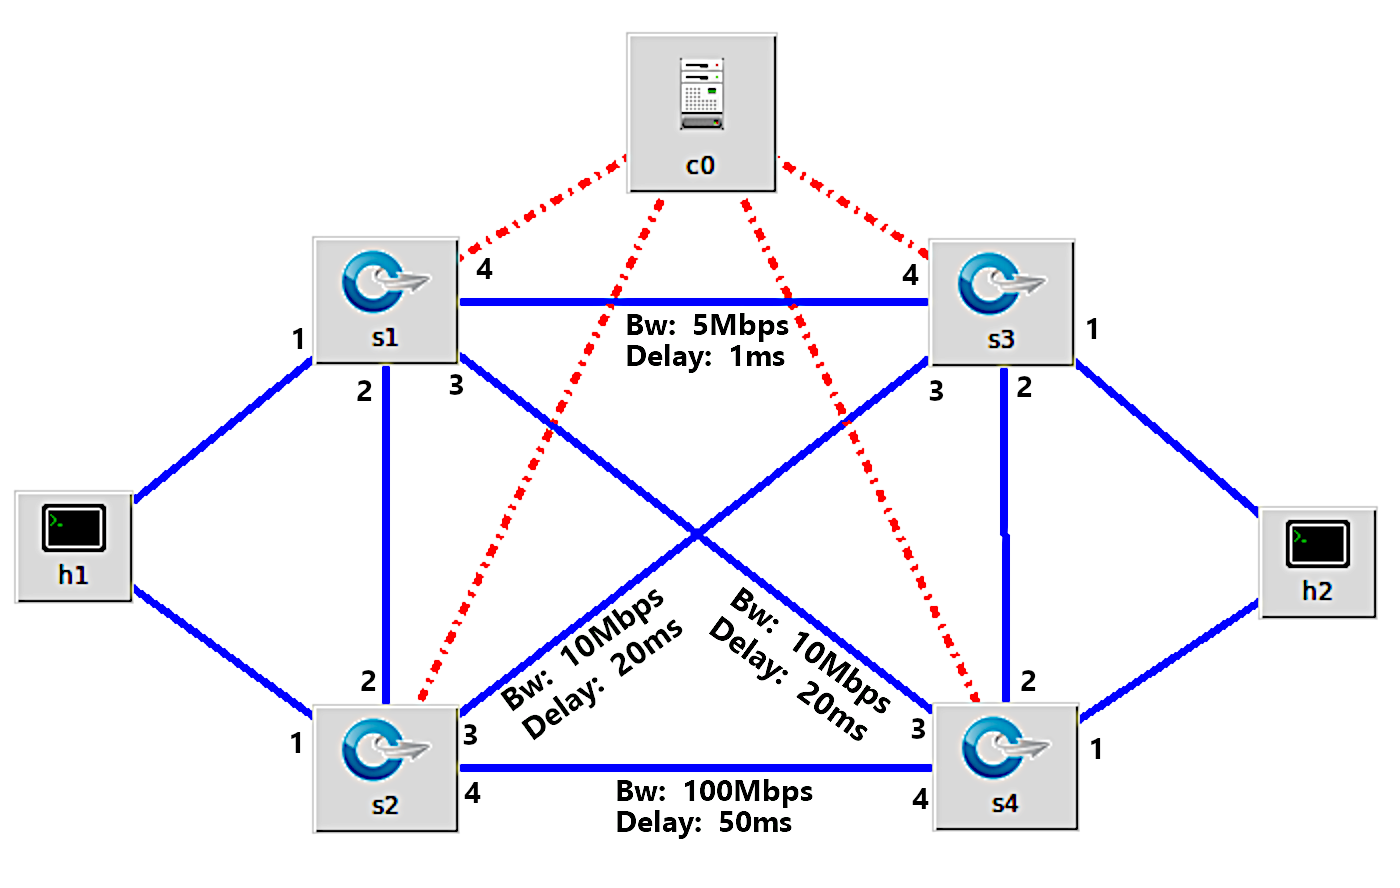
\includegraphics[width=1\linewidth]{../immagini/esempio/topo}
	\caption[Topologia d'esempio]{Topologia della rete in esame}
	\label{fig:topo}
\end{figure}
Come illustrato nel capitolo precedente, per costruire la topologia è necessario avvalersi di uno Script Python.\\Questo script verrà salvato nel file \textit{test.py}\\

\begin{lstlisting}[language=Python,numbers=left,firstnumber=1,stepnumber=1]
from mininet.topo import Topo
from mininet.link import TCLink
	
class MyTopo( Topo ):
	"Simple topology example."
	
	def __init__( self ):
		"Create custom topo."
	
		# Initialize topology
		Topo.__init__( self )
	
		# Add hosts and switches
		h1 = self.addHost( 'h1' )
		h2 = self.addHost( 'h2' )
		s1 = self.addSwitch( 's1' )
		s2 = self.addSwitch( 's2' )
		s3 = self.addSwitch( 's3' )
		s4 = self.addSwitch( 's4' )
	
		# Add links
		self.addLink( h1, s1, 1, 1, bw=100, delay='1ms' )
		self.addLink( h1, s2, 2, 1, bw=100, delay='1ms' )
		self.addLink( h2, s3, 1, 1, bw=100, delay='1ms' )
		self.addLink( h2, s4, 2, 1, bw=100, delay='1ms' )
		self.addLink( s1, s2, 2, 2, bw=100, delay='1ms' )
		self.addLink( s3, s4, 2, 2, bw=100, delay='1ms' )
		
		self.addLink( s1, s3, 4, 4, bw=5, delay='1ms' )
		self.addLink( s1, s4, 3, 3, bw=10, delay='20ms' )
		self.addLink( s2, s3, 3, 3, bw=10, delay='20ms' )
		self.addLink( s2, s4, 4, 4, bw=100, delay='50ms' )
	
topos = { 'mytopo': ( lambda: MyTopo() ) }
\end{lstlisting}
Possiamo notare alcune differenze con il codice di esempio fornito nel capitolo precedente.\\
Nella creazione dei link, infatti, viene specificate le porte di ciascun nodo a cui ciascun ramo è collegato.\\
Per le connessioni create nelle righe 29, 30, 31 e 32, inoltre, sono state specificate banda e latenza, coerentemente con i dati della figura 3.1, mentre per le altre sono stati scelti come parametri standard 100Mbps di banda e 1ms di latenza.\\
A causa di questa differenza, è necessario importare ulteriori API, operazione che viene svolta alla riga 2.\\\\
Ai fini della dimostrazione è necessario creare due reti distinte, una classica e una di tipo SDN. Lo script Python deve quindi essere eseguito in due modi diversi.
\begin{itemize}
	\item Per creare una topologia classica si usa il comando
	\begin{center}
		\textbf{sudo mn --custom test.py --topo mytopo --link tc}
	\end{center}
	che avvia Mininet con la topologia \textit{"mytopo"} del file \textit{"test.py"}\\
	Da notare il parametro \textit{--link} che deve essere posto \textit{"tc"} per permettere la personalizzazione di banda e latenza.\\
	\item Per creare una topologia SDN bisogna invece scrivere
	\begin{center}
		\textbf{sudo mn --custom test.py --topo mytopo --link tc --switch ovsk}
	\end{center}
	specificando quindi che gli switch debbano supportare OpenFlow.\\
\end{itemize}

\subsection{Forwarding}\label{ch:3.2.2}
È ora necessario configurare gli switch affinché la rete possa essere ottimizzata per i servizi richiesti.\\
Perchè avvenga è necessario che i pacchetti che richiedono una bassa latenza, rappresentati dai servizi sulla porta TCP 5000, siano inviati sul ramo che collega s1 a s3, mentre per i servizi che necessitano di molta banda, rappresentati dai pacchetti \textit{FTP}, è necessario che le informazioni viaggino sul ramo che collega s2 e s4.\\
I rami che collegano s1 con s2 e s3 con s4 sono dedicati a spostare i pacchetti verso il migliore tra i due percorsi.\\\\
Per configurare gli switch utilizziamo i comandi presentati nel capitolo precedente, con sintassi di questo tipo:\\
\begin{center}
	\textbf{ovs-ofctl add-flow [switch] priority=[priorità],in\_port=[porta switch],tcp,tcp\_src=[porta TCP],actions=output:[porta switch] }\\
\end{center}
Analizziamo il parametri del comando:\\
\begin{itemize}
	\item \textit{priority} definisce la priorità dell'azione. Un comando con priorità alta prevale su uno con priorità bassa.\\
	\item \textit{in\_port} specifica in quale porta dello switch debbano entrare i pacchetti appartenenti al flusso\\
	\item \textit{tcp\_src} specifica quale porta TCP stiano usando i pacchetti appartenenti al flusso\\
	\item \textit{output} definisce su quale porta dello switch dovranno essere reindirizzati i pacchetti in uscita\\
\end{itemize}
Per comodità, tutti i comandi necessari vengono racchiusi in uno script chiamato \textit{test.sh}, che presenta il seguente contenuto
\begin{lstlisting}[language=bash,numbers=left,firstnumber=1,stepnumber=1]
#Elimino i flussi preesistenti
sudo ovs-ofctl del-flows s1
sudo ovs-ofctl del-flows s2
sudo ovs-ofctl del-flows s3
sudo ovs-ofctl del-flows s4

#Creo un collegamento tra gli switch e i propri host
sudo ovs-ofctl add-flow s1 priority=1,actions=output:1
sudo ovs-ofctl add-flow s2 priority=1,actions=output:1
sudo ovs-ofctl add-flow s3 priority=1,actions=output:1
sudo ovs-ofctl add-flow s4 priority=1,actions=output:1

#Creo un canale di default
sudo ovs-ofctl add-flow s1 priority=2,in_port=1,actions=output:3
sudo ovs-ofctl add-flow s2 priority=2,in_port=1,actions=output:3
sudo ovs-ofctl add-flow s3 priority=2,in_port=1,actions=output:3
sudo ovs-ofctl add-flow s4 priority=2,in_port=1,actions=output:3

#Sposto i pacchetti verso le linee ottimizzate
sudo ovs-ofctl add-flow s1 
	priority=4,dl_type=0x0800,nw_proto=6,in_port=1,tcp,tcp_dst=20,
	actions=output:2
sudo ovs-ofctl add-flow s3 
	priority=4,dl_type=0x0800,nw_proto=6,in_port=1,tcp,tcp_dst=20,
	actions=output:2
sudo ovs-ofctl add-flow s2 
	priority=4,dl_type=0x0800,nw_proto=6,in_port=1,tcp,tcp_dst=5000,
	actions=output:2
sudo ovs-ofctl add-flow s4 	
	priority=4,dl_type=0x0800,nw_proto=6,in_port=1,tcp,tcp_dst=5000,
	actions=output:2

#Trasferisco i pacchetti sulle linee ottimizzate
sudo ovs-ofctl add-flow s1 
	priority=3,dl_type=0x0800,nw_proto=6,in_port=1,tcp,tcp_dst=5000,
	actions=output:4
sudo ovs-ofctl add-flow s3 
	priority=3,dl_type=0x0800,nw_proto=6,in_port=2,tcp,tcp_dst=5000,
	actions=output:4
sudo ovs-ofctl add-flow s2 
	priority=3,dl_type=0x0800,nw_proto=6,in_port=2,tcp,tcp_dst=20,
	actions=output:4
sudo ovs-ofctl add-flow s4 
	priority=3,dl_type=0x0800,nw_proto=6,in_port=1,tcp,tcp_dst=20,
	actions=output:4

sudo ovs-ofctl dump-flows s1
sudo ovs-ofctl dump-flows s2
sudo ovs-ofctl dump-flows s3
sudo ovs-ofctl dump-flows s4
\end{lstlisting}
Per avviare lo script è necessario renderlo eseguibile. Per farlo bisogna scrivere nella CLI
\begin{center}
	\textbf{sudo chmod +X \textit{test.sh}}
\end{center}
Il comando per avviare lo script invece è
\begin{center}
	\textbf{sudo bash ./\textit{test.sh}}
\end{center}
Le righe tra 2 e 5 servono per eliminare eventuali flussi preesistenti.\\
Le righe tra 8 e 17 creano un collegamento di default, per permettere ai servizi sconosciuti di poter giungere a destinazione.\\
I comandi nelle righe tra 20 e 31 servono per permettere ai pacchetti di giungere sulla linea più adatta al servizio richiesto.\\
Le righe tra 34 e 45 compiono il vero e proprio trasferimento delle informazioni sulla linea. Una volta giunte allo switch successivo, queste vengono portate all'host grazie ai flussi precedentemente creati.\\\\
Per analizzare come le prestazioni vengano modificate dalla programmazione della rete misuriamo latenza e banda della rete per i diversi servizi prima e dopo l'esecuzione dello script.\\
Per un corretto inoltro delle informazione attraverso gli switch anche senza una programmazione tramite controller è necessario attivare l'\textit{STP (Spanning Tree Protocol)}, che permette alla rete di stabilire un percorso per collegare i due host, interrompendo gli altri collegamenti.\\
Se si prova ad usare il comando \textit{pingall} subito dopo aver costruito la topologia, infatti, possiamo notare che gli host non sono in grado di comunicare.\\
\begin{figure}[H]
	\centering
	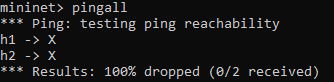
\includegraphics[width=0.9\linewidth]{../immagini/esempio/stp_off}
	\caption[Pingall con STP disattivato]{Il comando "pingall" ci permette di vedere che gli host non riescono ad inviarsi informazioni}
	\label{fig:stpoff}
\end{figure}
È quindi necessario attivare l'STP. Per farlo, bisogna usare uno specifico comando, anche in questo caso presentato in uno script per semplicità.\\
\begin{lstlisting}[language=bash]
sudo ovs-vsctl set Bridge 's1' stp_enable=true
sudo ovs-vsctl set Bridge 's2' stp_enable=true
sudo ovs-vsctl set Bridge 's3' stp_enable=true
sudo ovs-vsctl set Bridge 's4' stp_enable=true
\end{lstlisting}
Una volta attivato l'STP, la rete stabilisce un percorso tra i due host, che riescono finalmente a comunicare. Tuttavia, è importante notare che, così facendo, la maggior parte delle risorse rimangono inutilizzate.\\\\
Come sarà evidente in fase di analisi prestazionale, il collegamento tra i due host può coincidere con uno dei percorsi della rete SDN.\\
Tuttavia, gli aspetti che si vogliono evidenziare con questa dimostrazione non sono le differenze delle prestazioni in senso assoluto, ma l'incapacità di una rete classica di adattarsi allo specifico servizio richiesto.\\\\
Possiamo riutilizzare il comando \textit{pingall} per testare nuovamente il funzionamento della rete.
\begin{figure}[H]
	\centering
	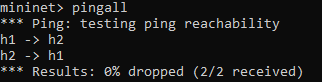
\includegraphics[width=0.9\linewidth]{../immagini/esempio/stp_on}
	\caption[Pingall con STP attivato]{Dopo aver attivato l'STP esiste un percorso tra i due host}
	\label{fig:stpon}
\end{figure}

\section{Prestazioni}\label{ch:3.3}
Avendo a disposizione la rete programmata ed un'alternativa non ottimizzata, è possibile raccogliere dei dati riguardanti le prestazioni tramite gli strumenti presentati nel capitolo precedente.
\subsection{Latenza}\label{ch:3.3.1}
\begin{figure}[H]
	\centering
	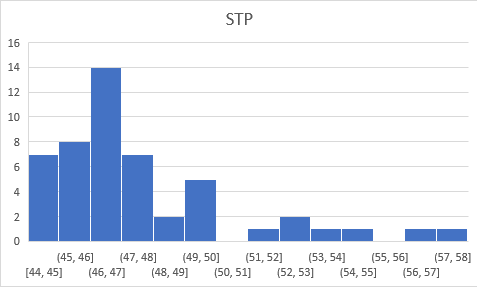
\includegraphics[width=0.9\linewidth]{../immagini/esempio/ping_stp}
	\caption[Latenza STP]{Latenza misurata su 50 misurazioni con la topologia basata su STP}
	\label{fig:pingstp}
\end{figure}
\begin{figure}[H]
	\centering
	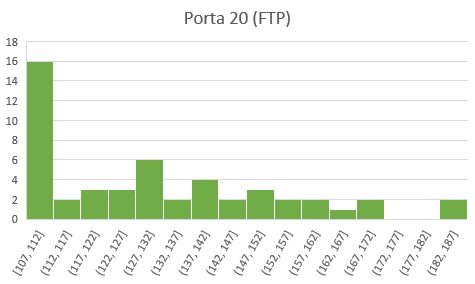
\includegraphics[width=0.9\linewidth]{../immagini/esempio/ping_ftp}
	\caption[Latenza Porta 20]{Latenza misurata su 50 misurazioni con il percorso ottimizzato per la porta 20}
	\label{fig:pingftp}
\end{figure}
\begin{figure}[H]
	\centering
	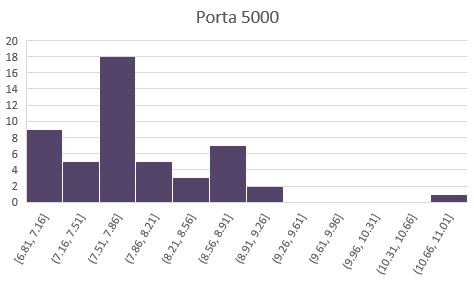
\includegraphics[width=0.9\linewidth]{../immagini/esempio/ping_5000}
	\caption[Latenza Porta 5000]{Latenza misurata su 50 misurazioni con il percorso ottimizzato per la porta 5000}
	\label{fig:ping5000}
\end{figure}
\begin{figure}[H]
	\centering
	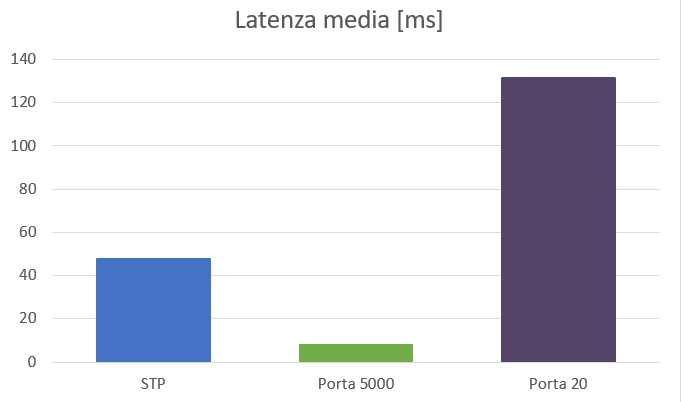
\includegraphics[width=0.9\linewidth]{../immagini/esempio/ping_medio}
	\caption[Latenza media]{Latenza media misurata su 50 misurazioni per ogni servizio}
	\label{fig:pingmedio}
\end{figure}
Possiamo osservare che il percorso stabilito tramite Spanning Tree Protocol coincide con il percorso che, nella rete programmata, viene svolto dai pacchetti di servizi non specificati.\\
\subsection{Banda}\label{ch:3.3.2}
\begin{figure}[H]
	\centering
	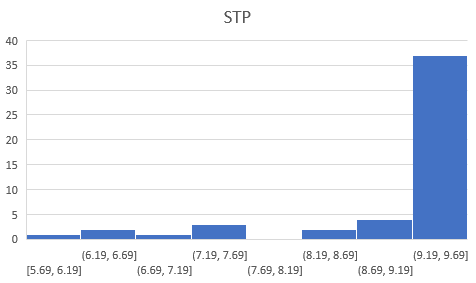
\includegraphics[width=1\linewidth]{../immagini/esempio/bw_stp}
	\caption[Banda STP]{Banda misurata su 50 misurazioni con la topologia basata su STP}
	\label{fig:bwstp}
\end{figure}
\begin{figure}[H]
	\centering
	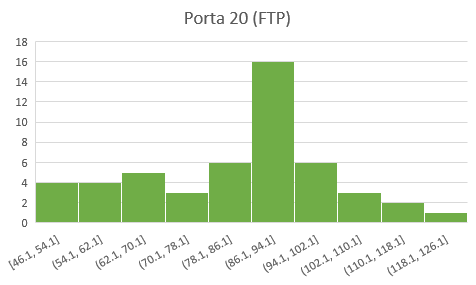
\includegraphics[width=1\linewidth]{../immagini/esempio/bw_ftp}
	\caption[Banda Porta 20]{Banda misurata su 50 misurazioni con il percorso ottimizzato per la porta 20}
	\label{fig:bwftp}
\end{figure}
\begin{figure}[H]
	\centering
	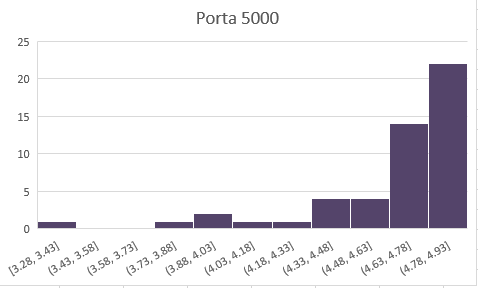
\includegraphics[width=1\linewidth]{../immagini/esempio/bw_5000}
	\caption[Banda Porta 5000]{Banda misurata su 50 misurazioni con il percorso ottimizzato per la porta 5000}
	\label{fig:bw5000}
\end{figure}
\begin{figure}[H]
	\centering
	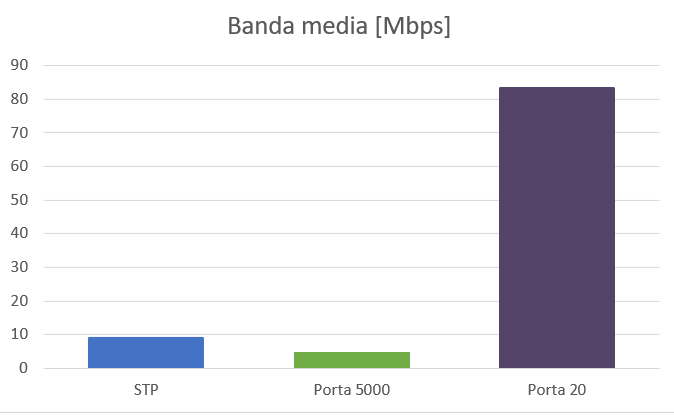
\includegraphics[width=1\linewidth]{../immagini/esempio/bw_media}
	\caption[Banda media]{Banda media misurata su 50 misurazioni per ogni servizio}
	\label{fig:bwmedia}
\end{figure}

È possibile notare come le prestazioni della rete standard non siano necessariamente peggiori rispetto alla rete programmata. È importante però osservare come queste non dipendano dallo specifico servizio richiesto e non siano quindi in grado di accontentare al meglio le diverse esigenze.